The classification scheme as described above has been used on the Banknote Authentication dataset \cite{banknote_paper} (downloaded from \cite{banknote_download}\footnote{Note that this page explains the labels the wrong way around. See \cite{genuine_class_banknote}}).
This particular dataset was chosen because it required only few particles to encode the input and the output:
\begin{enumerate}
	\item There are only two distinct labels (binary classification).
	\item Each input vector contains only four elements.
\end{enumerate}

The implementation is available at \url{https://github.com/Nifrec/nenwin} under the open-source AGPL-3.0 licence\cite{AGPL_3}.

Note that these experiments are intended to give an indication of trainability and parameter sensitivity of the \textsc{Nenwin} framework. 
A full search-space evaluation is beyond the scope of this report (and would require a more optimized implementation).

\subsection{Dataset description}
The classification task is to classify banknotes as genuine or as forgeries, 
given four derived features from the images. 
Class 0 has 762 samples and represent the genuine banknotes,
class 1 has 610 represents the forgeries. 
This split is close to a 50\%/50\% split, meaning that random classification would yield an accuracy around 50\%.
The derived features (of Wavelet-transformed image) have been pre-computed, and are:
\begin{enumerate}
	\item Variance
	\item Skewness
	\item Kurtosis
	\item Entropy
\end{enumerate}

For the experiments, the samples of the dataset were shuffled in a random order and split in a 80\%/10\%/10\% train/validation/test set split. 
This split was cached and reused for each experiment (i.e. each experiment had the same train, validation and test set).

\subsection{Architectures}
Three different architectures have been designed and were evaluated. See also Fig. \ref{fig:banknote_architectures}.

In all architectures, all Nodes have their mass, \texttt{marble\_stiffness},
\texttt{node\_stiffness} and \texttt{marble\_attraction} set to 1, 
and their \texttt{node\_attraction} to 0. 
Note that these are only initial values for learnable parameters. 
The MarbleEaterNodes had their radius set to 0.5, which was not optimized by the implementation.

\paragraph{Architecture A:}
\begin{itemize}
	\item Vertices of input region: (-2.5, -1), (-2.5, 1), (2.5, -1), (2.5, 1).
	\item 4 non-output nodes surrounding the input region (positions (0, -5), (-5, 0), (5, 0) and (0, 5)).
	\item MarbleEaterNodes (output Nodes) at (-10, 0) and (10, 0).
\end{itemize}

\paragraph{Architecture B:}
Same as Architecture A, but with additional Nodes at (2.5, 2.5), (-2.5, 2.5), (2.5, -2.5), (-2.5, -2.5).

\paragraph{Architecture C:}
\begin{itemize}
	\item Vertices of input region: (0, 0), (0, 1), (6, 0), (6, 1).
	\item 5 non-output nodes surrounding the input region (positions (1, 2), (2, 3), (3, 2), (4, 3) and (5, 2)).
	\item MarbleEaterNodes (output Nodes) at (1, 4) and (5, 4).
\end{itemize}

\begin{figure}
	\centering
	\begin{subfigure}[b]{0.3\textwidth}
		\centering
		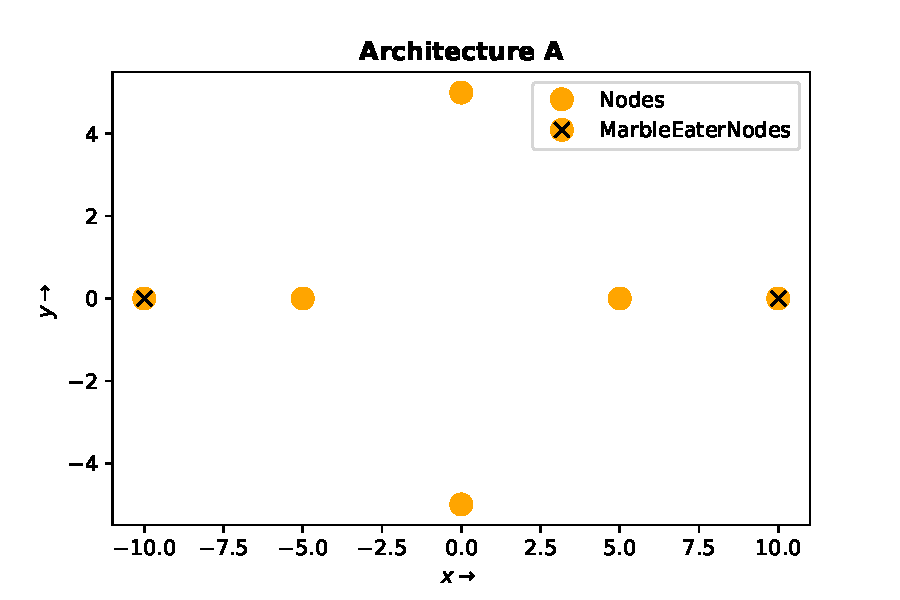
\includegraphics[width=\textwidth]{figures/architecture_A.pdf}
		\label{fig:architecture_a}
	\end{subfigure}
	\begin{subfigure}[b]{0.3\textwidth}
		\centering
		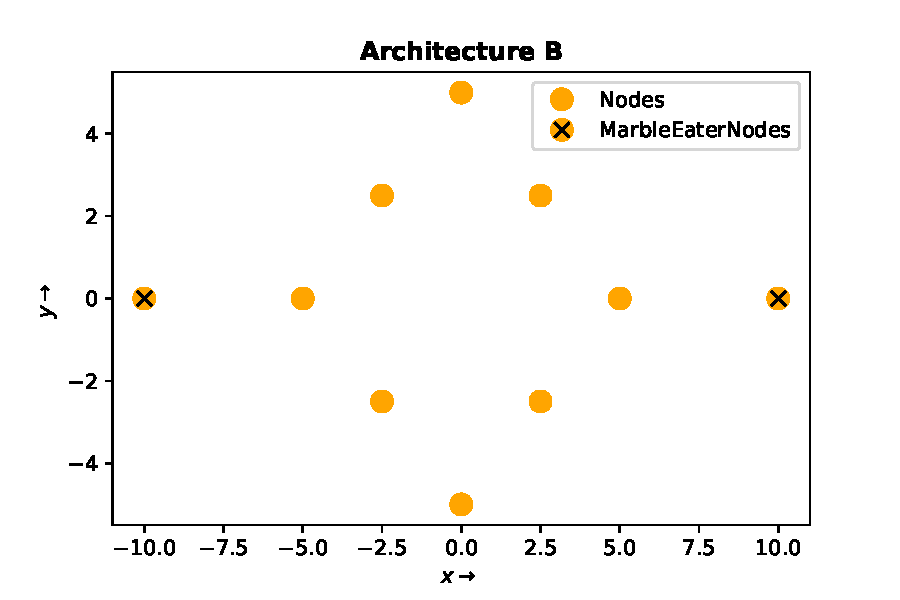
\includegraphics[width=\textwidth]{figures/architecture_B.pdf}
		\label{fig:architecture_b}
	\end{subfigure}
	\begin{subfigure}[b]{0.3\textwidth}
		\centering
		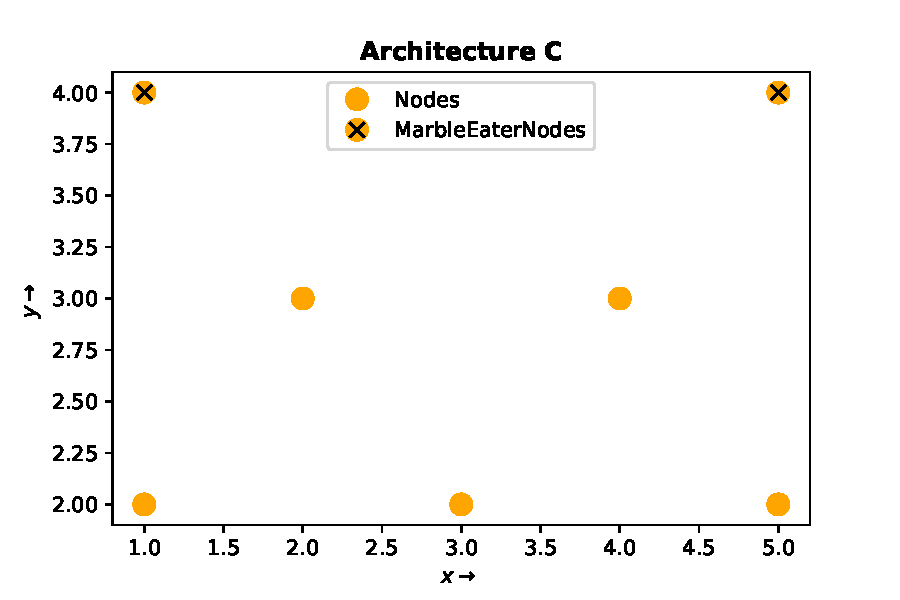
\includegraphics[width=\textwidth]{figures/architecture_C.pdf}
		\label{fig:architecture_c}
	\end{subfigure}

	\caption{\textsc{Nenwin} Architectures used for training on the banknote dataset.}
	\label{fig:banknote_architectures}
\end{figure}

\subsection{Setup}
For each experiment, one of the architectures A, B or C was generated, and other hyperparameters were chosen.
In particular, the batch size and the input placer were varied. 

The training procedure used was as follows:
during each epoch, the samples of the training set are iterated in a random order. 
Each sample in the training set converted to Marbles by the chosen input placer.
Then the simulation is run until at least one MarbleEaterNode ate a Marble, 
or until a maximum number of steps is reached. 
Then the loss is computed according to \eqref{eq:classification_loss_full},
and gradients of parameters with respect to this loss are computed via backpropagation.
Finally the parameters are updated using the Adam optimization technique \cite{adam}.

The average gradients over the batch are used in case the batch size is larger than 1. 
The samples are still processed in sequential order, but the gradients of their losses are accumulated.
The Adam update rule is only used after the last sample in the batch.

The value of $\mu$ in \eqref{eq:classification_loss_one_marble} was set to 1. 
Newton's gravity function (without gravitation constant, 
\eqref{eq:newton_grav_force}) was used as the attraction function for all particles. 
For all Marbles, 
both the \texttt{marble\_stiffness} and \texttt{node\_attraction} were set to 1,
and both the \texttt{node\_stiffness} and \texttt{marble\_attraction} to 0. 



Because of practical resource and time constraints, this maximum amount of timesteps was set to only 20 steps, with a stepsize of 0.1. 
With this configuration it took several hours to train an architecture\footnote{Training was run on a a Intel(R) Core(TM) i7-7700HQ CPU @ 2.80GHz.}. 

\subsection{Results}

Numerical results of various training-runs have been summarized in Table \ref{table:banknote_exp}. 

\begin{table}[hb]
	\begin{tabular}{lll|lll}
		\textbf{Architecture} &
		\textbf{Timesteps} &
		\textbf{\begin{tabular}[c]{@{}l@{}}input\\ placer\end{tabular}} &
		\textbf{\begin{tabular}[c]{@{}l@{}}batch\\ size\end{tabular}} &
		\textbf{\begin{tabular}[c]{@{}l@{}}validation\\ accuracy\end{tabular}} &
		\textbf{\begin{tabular}[c]{@{}l@{}}training\\ loss\end{tabular}} \\ \hline
		A & 20 & VelInputPlacer  & 1 & 0.17518 & 20307.7 \\
		A & 20 & VelInputPlacer  & 2 & 0.13869 & 21173.4 \\
		A & 20 & VelInputPlacer  & 5 & 0.06569 & 28580.8 \\
		A & 20 & MassInputPlacer & 1 & 0.0     & 13.5    \\
		C & 20 & MassInputPlacer($\begin{bmatrix} 1\\1\end{bmatrix}$) & 1 & 0.0 & 200.1 \\
		B & 20 & VelInputPlacer  & 2 & 0.12409 & 24788.9 \\
		C & 20 & VelInputPlacer  & 2 & 0.08029 & 33143.6 \\
		C & 40 & MassInputPlacer($\begin{bmatrix} 0.5\\0\end{bmatrix}$) & 1 & 0.0 & 107.6 \\
		C & 36 & MassInputPlacer($\begin{bmatrix} 0.5\\0\end{bmatrix}$) & 2 & \textbf{0.51825} & -1198.1 \\
		C & 40 & MassInputPlacer($\begin{bmatrix} 0.5\\0\end{bmatrix}$) & 2 & 0.20438 & -4590.7
	\end{tabular}
	\caption{Results of training a \nenwin architecture on the banknote-authentication dataset. Each row represents an independent training run. The accuracy is the total amount of correct predictions divided over the size of the validation set. Absence of output is counted as a wrong prediction. The loss accumulation of losses of the last epoch of the train set.}
	\label{table:banknote_exp}
\end{table}

Most hyperparameter-configurations appear to provide poor results. 
A plot of the performance per epoch shows that the training initially makes progress, 
see Fig. \ref{fig:velinputplacer_performance}. 
The loss decreases roughly exponential during the first epochs, and the validation accuracy roughly increases logarithmically. 
However, the training progress converges too quickly to mediocre performance. 

One possible explanation for the poor performance of the VelInputPlacer, 
is that it gives the input Marbles a high initial velocity in varying directions. 
With a very limited amount of Nodes,
the model may not possess the flexibility handle all combinations of initial velocity directions of the Marbles. 

\begin{figure}[hb]
	\centering
	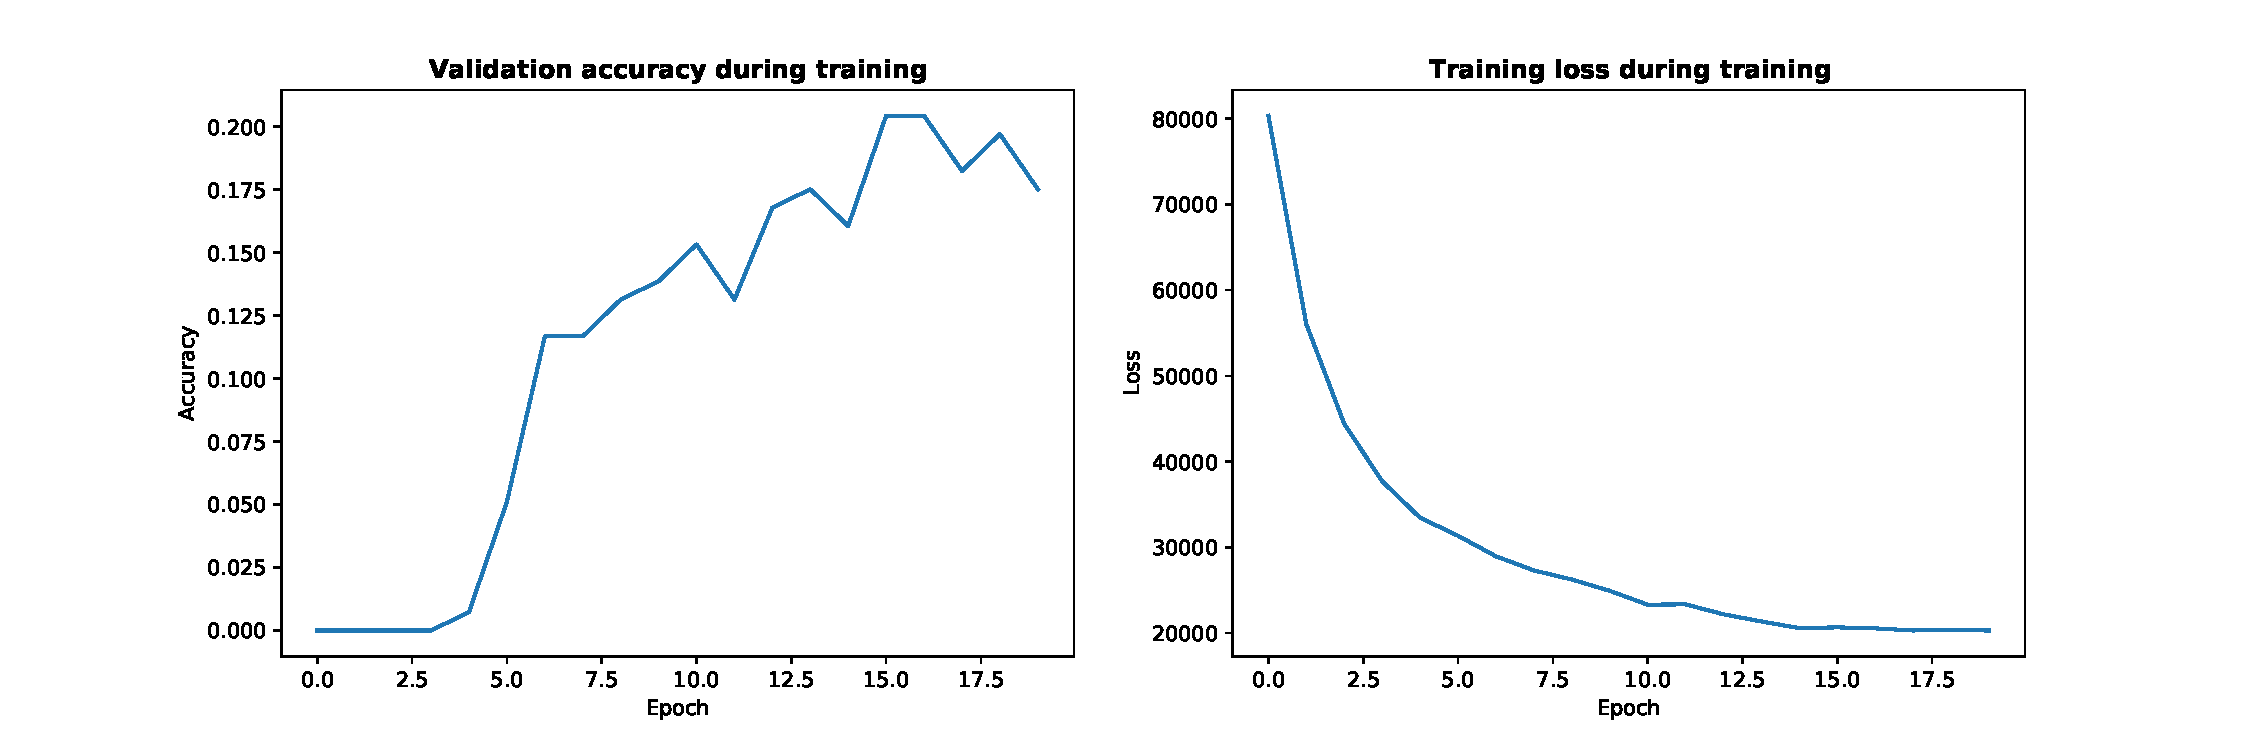
\includegraphics[scale=0.4]{figures/A_batch1_velinputplacer.pdf}
	\caption{Performance of Architecture A as measured during each epoch of training. The VelInputPlacer was used to map the four banknote features to four Marbles. The batch size was 1. Note how the improvement of the accuracy on the validation set already seems to destabilize and cease rapid growth in less than 20 epochs. Given that the decrease in train set loss also flattened out at this time, it would seem unlikely that running more epochs would significantly increase the validation set accuracy.}
	\label{fig:velinputplacer_performance}
\end{figure}

\clearpage

\subsubsection{Evaluation best run}
The most surprising results are obtained with the MassInputPlacer with a velocity vector of $\begin{bmatrix} 0.5\\0\end{bmatrix}$, 
a batch size of 2, and using Architecture C as initial architecture. 
Note that Marbles will be moving towards the MarbleEaterNodes with this initial velocity in Architecture C. 
After 36 epochs this resulted in a validation-set accuracy above chance level, see Fig. \ref{fig:arch_c_const_vel_50pc_learning_curve}. 
However, the learning curve shows very eccentric patterns. 
The high validation set accuracy after 36 epochs quickly disappeared after more epochs. 
This might be due to overfitting, although it is a very sudden change. 
The high non-convexity of the training objective may be a more likely explanation. 

One hypothesis is that the optimization rule might have stepped a bit too far in a certain direction (by updating the parameters), 
and entered the domain of the loss function which has a different local minimum. 
This is for example possible if the optimization step caused a small adjustment that made a Marble being eaten early in the simulation, 
which would otherwise bypass the MarbleEaterNode. This would change the moment that the loss in computed. 
This may result in a very different loss, as the other Marbles will be at very different positions than at the end of the maximum simulation time.
The Marble $m'$ that was eaten may change the loss directly. 
If $m'$ was eaten by a MarbleEaterNode $n'$ (and $n'$ represents the wrong prediction), 
then a new term $- \frac{1}{f(m', n', t_{end})}$ will be included to the loss. 
Since the distance of $m'$ to $n'$ will be very small, $f(m', n', t_{end})$ will be small,
and the magnitude of the reciprocal term will be large.

The train-set loss also shows an extreme outlier, which occurs at the first epoch in the accuracy on the validation set experienced a sudden increase. 

Also see Fig. \ref{fig:arch_c_const_vel_50pc_architecture} for a comparison of Architecture C before and after 40 epochs of training. The architecture has changed significantly. The output Nodes have been moved towards the input region. Also the mass of all Nodes has been decreased, among with some of the \texttt{attraction}- and \texttt{stiffness}-parameters (no Node had an increase). For example, the two MarbleEaterNodes had masses of 0.0753 and 0.0249\footnote{Rounded to four figures. Also the other parameter values in this paragraph have been rounded to four figures.} (the starting values were both 1). But the normal Nodes had much higher masses: as high as 0.7981 (the lowest was 0.0981).

The same pattern was observed for the \texttt{marble\_attraction}: 
it was much lower for the MarbleEaterNodes (0.0753 and 0.0015) 
than for the other Nodes 
(max: 0.7409, min: 0.0981, corresponding to the same 'normal' Nodes as the max and min mass).
Apparently the model had learned that output Nodes should attract Marbles less strongly, 
as both the mass and the \texttt{marble\_attraction} are used to compute the attraction force Marbles experience.

The \texttt{marble\_stiffness} remained close to 1 for most Nodes: 
only 1 'normal' Node had an extremely low value of 0.2775, 
and one MarbleEaterNode 0.5573 (for all others it was above 0.84). 
Apparently, the model did not learn to keep all Nodes stationary. 

The test set score of this model, as obtained after 40 epochs, is 0.2174.
The corresponding loss is -24058.3422 (both numbers are rounded to four figures). 
This is very close to the performance on the validation set. 

\begin{figure}[hb]
	\centering
	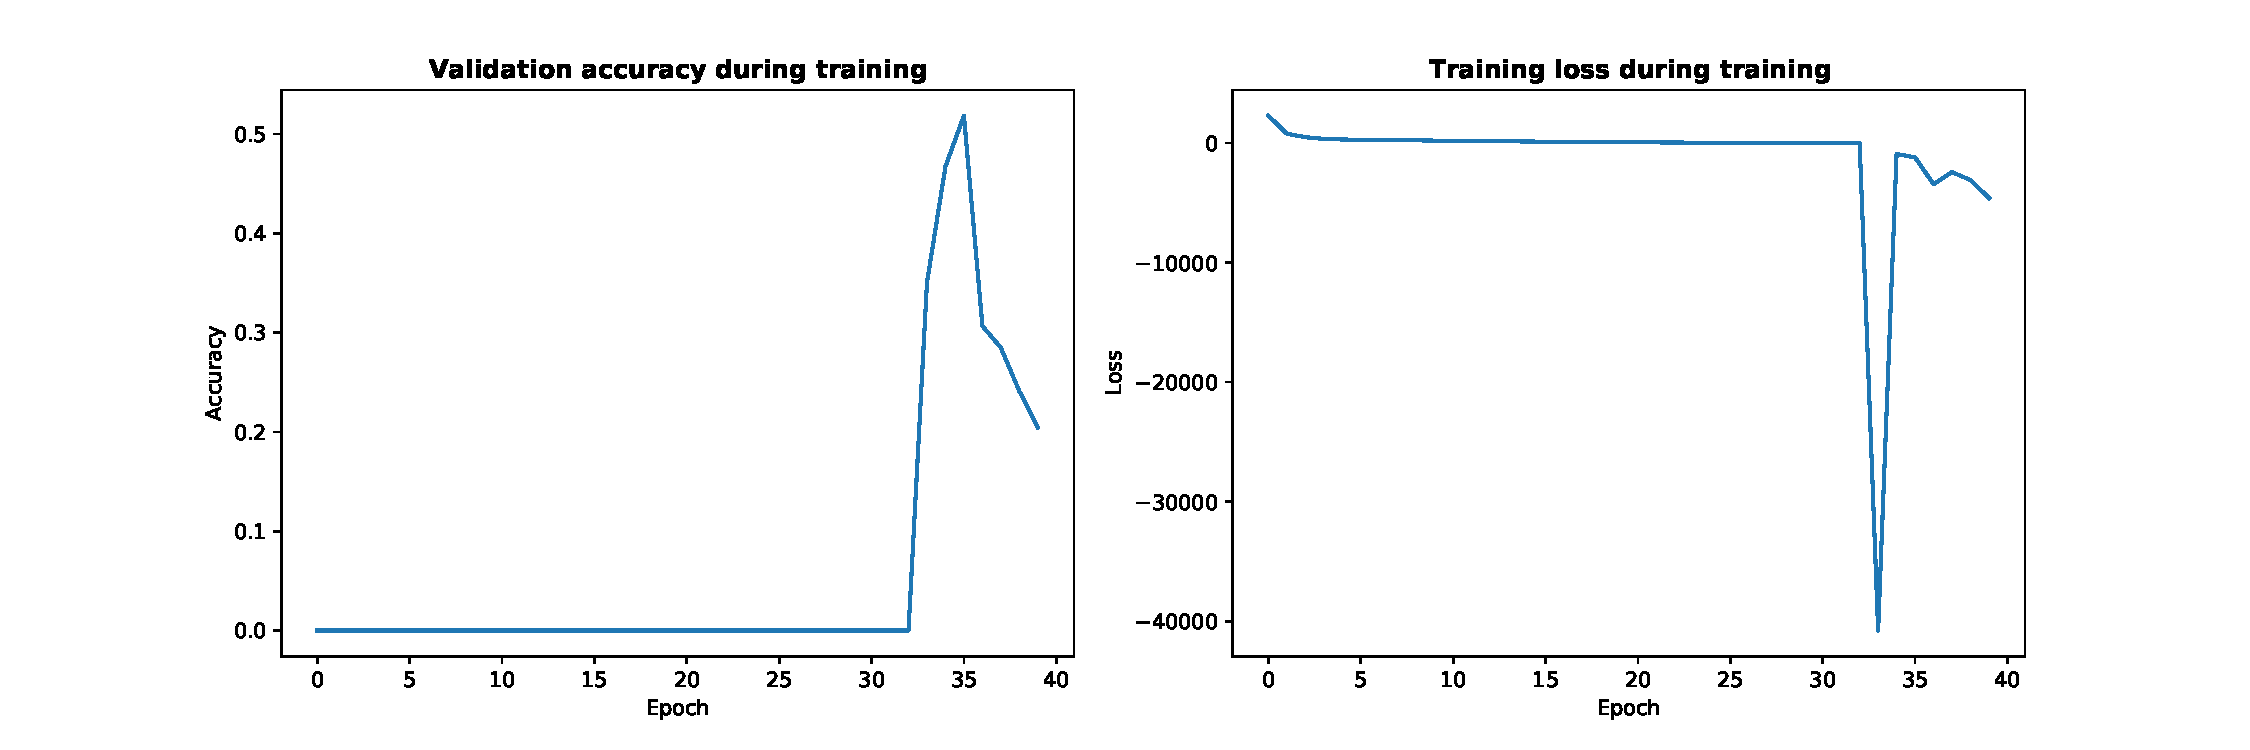
\includegraphics[scale=0.4]{figures/C_batch1_ConstVelInputPlacer([0.5, 0]])_epoch40_stats.pdf}
	\caption{Learning curves of using Architecture C with 
		a batch size of 2, MassInputPlacer($\begin{bmatrix} 0.5\\0\end{bmatrix}$) and 40 train-set epochs.}
	\label{fig:arch_c_const_vel_50pc_learning_curve}
\end{figure}

\begin{figure}[hb]
	\centering
	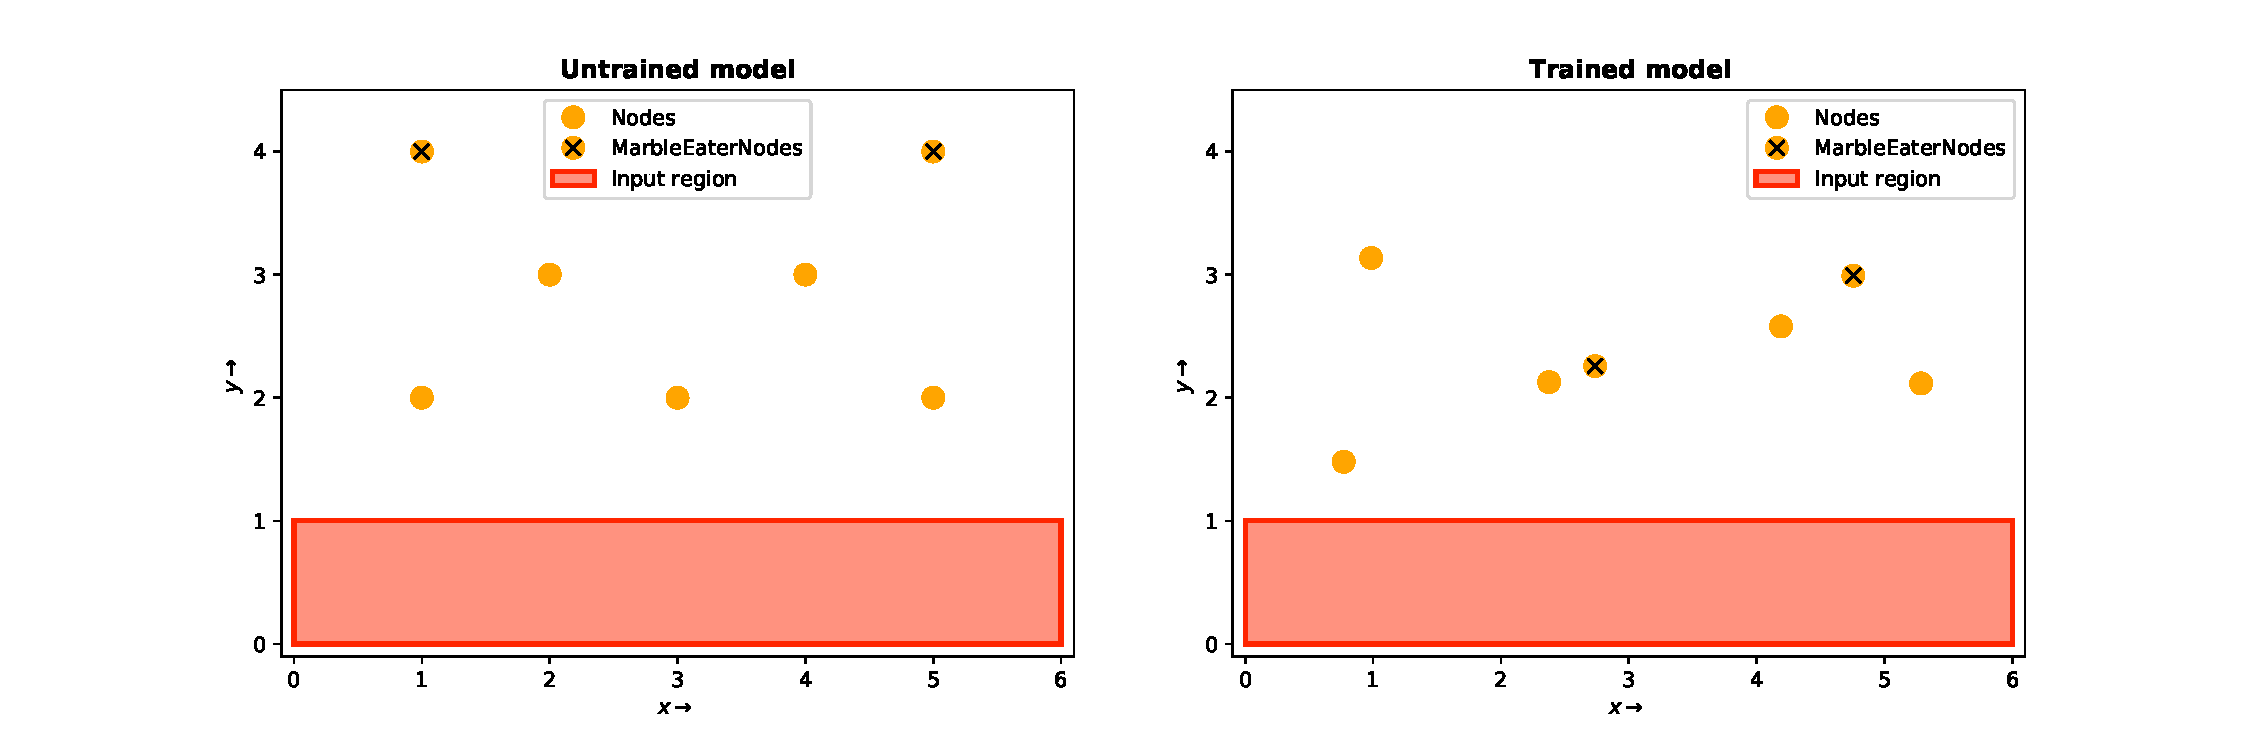
\includegraphics[scale=0.4]{figures/C_batch1_ConstVelInputPlacer([0.5, 0]])_epoch40.pdf}
	\caption{Architecture C before training (left) and after training on 40 epochs with 
		a batch size of 2, MassInputPlacer($\begin{bmatrix} 0.5\\0\end{bmatrix}$).}
	\label{fig:arch_c_const_vel_50pc_architecture}
\end{figure}

\clearpage